%%%%%%%%%%%%%%%%%%%%%%%%%%%%%%%%%%%%%%%%%%%%%%%%%%%%%%%%%%%%%%%%%%%%%%%%%%%%%%%%
% Лабораторная работа 6 : Определение линейных и угловых перемещений балки.
% Выполнили             : Баталов Семен, Хайретдинова Диана, 2021.
%%%%%%%%%%%%%%%%%%%%%%%%%%%%%%%%%%%%%%%%%%%%%%%%%%%%%%%%%%%%%%%%%%%%%%%%%%%%%%%%

\documentclass[12pt, a4paper]{article}
\usepackage[left=1.5cm, right=2cm, top=2.5cm, bottom=2.5cm, nohead]{geometry}
\usepackage{graphicx}
\usepackage[utf8]{inputenc}
\usepackage[english, russian]{babel}
\usepackage{indentfirst}
\usepackage{amsmath}
\usepackage{multirow}
\usepackage{array}
\usepackage{rotating}
\usepackage{subcaption}
\graphicspath{{./Figures/}}

\begin{document}
    
    \newcolumntype{M}[1]{>{\centering\arraybackslash}m{#1}}
    \renewcommand{\arraystretch}{1.3}
    
    \begin{center}
        \large{Санкт-Петербургский Государственный Университет} \\
        \large{Saint-Petersburg State University}\\
        \hfill \break
        \hfill \break
        \hfill \break
        \hfill \break
        \hfill \break
        \hfill \break
        \large{ЛАБОРАТОРИЯ ПРОЧНОСТИ МАТЕРИАЛОВ} \\
        \hfill \break
        \hfill \break
        \hfill \break
        \large{\textbf{ОТЧЕТ}} \\
        \large{\textbf{По лабораторной работе 6}} \\
        \large{<<Определение линейных и угловых перемещений балки>>} \\
        \hfill \break
        \hfill \break
        \hfill \break
        \large{По дисциплине} \\
        \large{<<Лабораторный практикум, лабораторная работа>>} \\
    \end{center}
    
    \hfill \break
    \hfill \break
    \hfill \break
    \hfill \break
    \hfill \break
    \hfill \break
    
    \begin{flushright} 
        \large{Выполнили:} \\
        \hfill \break
        \large{Баталов С. А.} \\
        \large{Хайретдинова Д. Д.} \\
    \end{flushright}
    
    \hfill \break
    \hfill \break
    \hfill \break
    \hfill \break
    \hfill \break
    
    \begin{center} 
        \large{Санкт-Петербург} \\
        \large{2021} \\
    \end{center}
    
    \thispagestyle{empty}
    \newpage
    \sloppy
    
    \section{Цель работы}
    
    Под изгибом понимают такой вид деформации, при котором в поперечных сечениях исследуемого образца возникают изгибающие моменты. Стержень, работающий на изгиб, называют балкой. Балка называется статически определимой, если все усилия и моменты в ней можно определить из уравнения статики. В частности, используемая в работе балка с одной шарнирно-подвижной и одной шарнирно-неподвижной опорами является статически определимой.
    
    При прямом поперечном изгибе ось бруса, искривляясь, остается в силовой плоскости. В результате деформации каждое из сечений занимает новое положение: их центры тяжести получают вертикальные и горизонтальные линейные перемещения, а сами сечения поворачивается на некоторый угол вокруг нейтральной оси. Гипотеза плоских сечений~--~при повороте сечения остаются плоскими и перпендикулярными изогнутой оси балки.
    
    Цель работы заключается в измерении линейных и угловых перемещений, возникающих в статически определимой шарнирно закрепленной балке при изгибе ее сосредоточенной силой и сравнении измеренных величин с расчетными данными.
    
    \newpage
    
    \section{Экспериментальная установка}
    
    Установка (рис.~\ref{im1}) выполнена в настольном исполнении и состоит из сварного основания \textit{1}, на котором закреплены стойки \textit{2} и \textit{3} в виде усеченной пирамиды. На стойках устанавливается контрольная балка \textit{4}, правый конец которой располагается на шарнирно-подвижной опоре \textit{5}, а левый конец на шарнирно-неподвижной опоре \textit{6}. Нагружение балки осуществляется через подвес \textit{7} с грузами. На балке нанесены риски с интервалом 50~мм для измерения расстояний при выполнении работы. Линейные перемещения (прогибы) измеряются индикаторной головкой \textit{8} часового типа, закрепленной на горизонтальной планке \textit{9}. Для измерения угловых перемещений опор балки используются индикаторные головки \textit{10}, закрепленные на рычаге \textit{11}. Расстояние между опорами $700 \pm 2~\text{мм}$. Балка выполнена из стали 45.
    
    \begin{figure}[h]
        \centering
        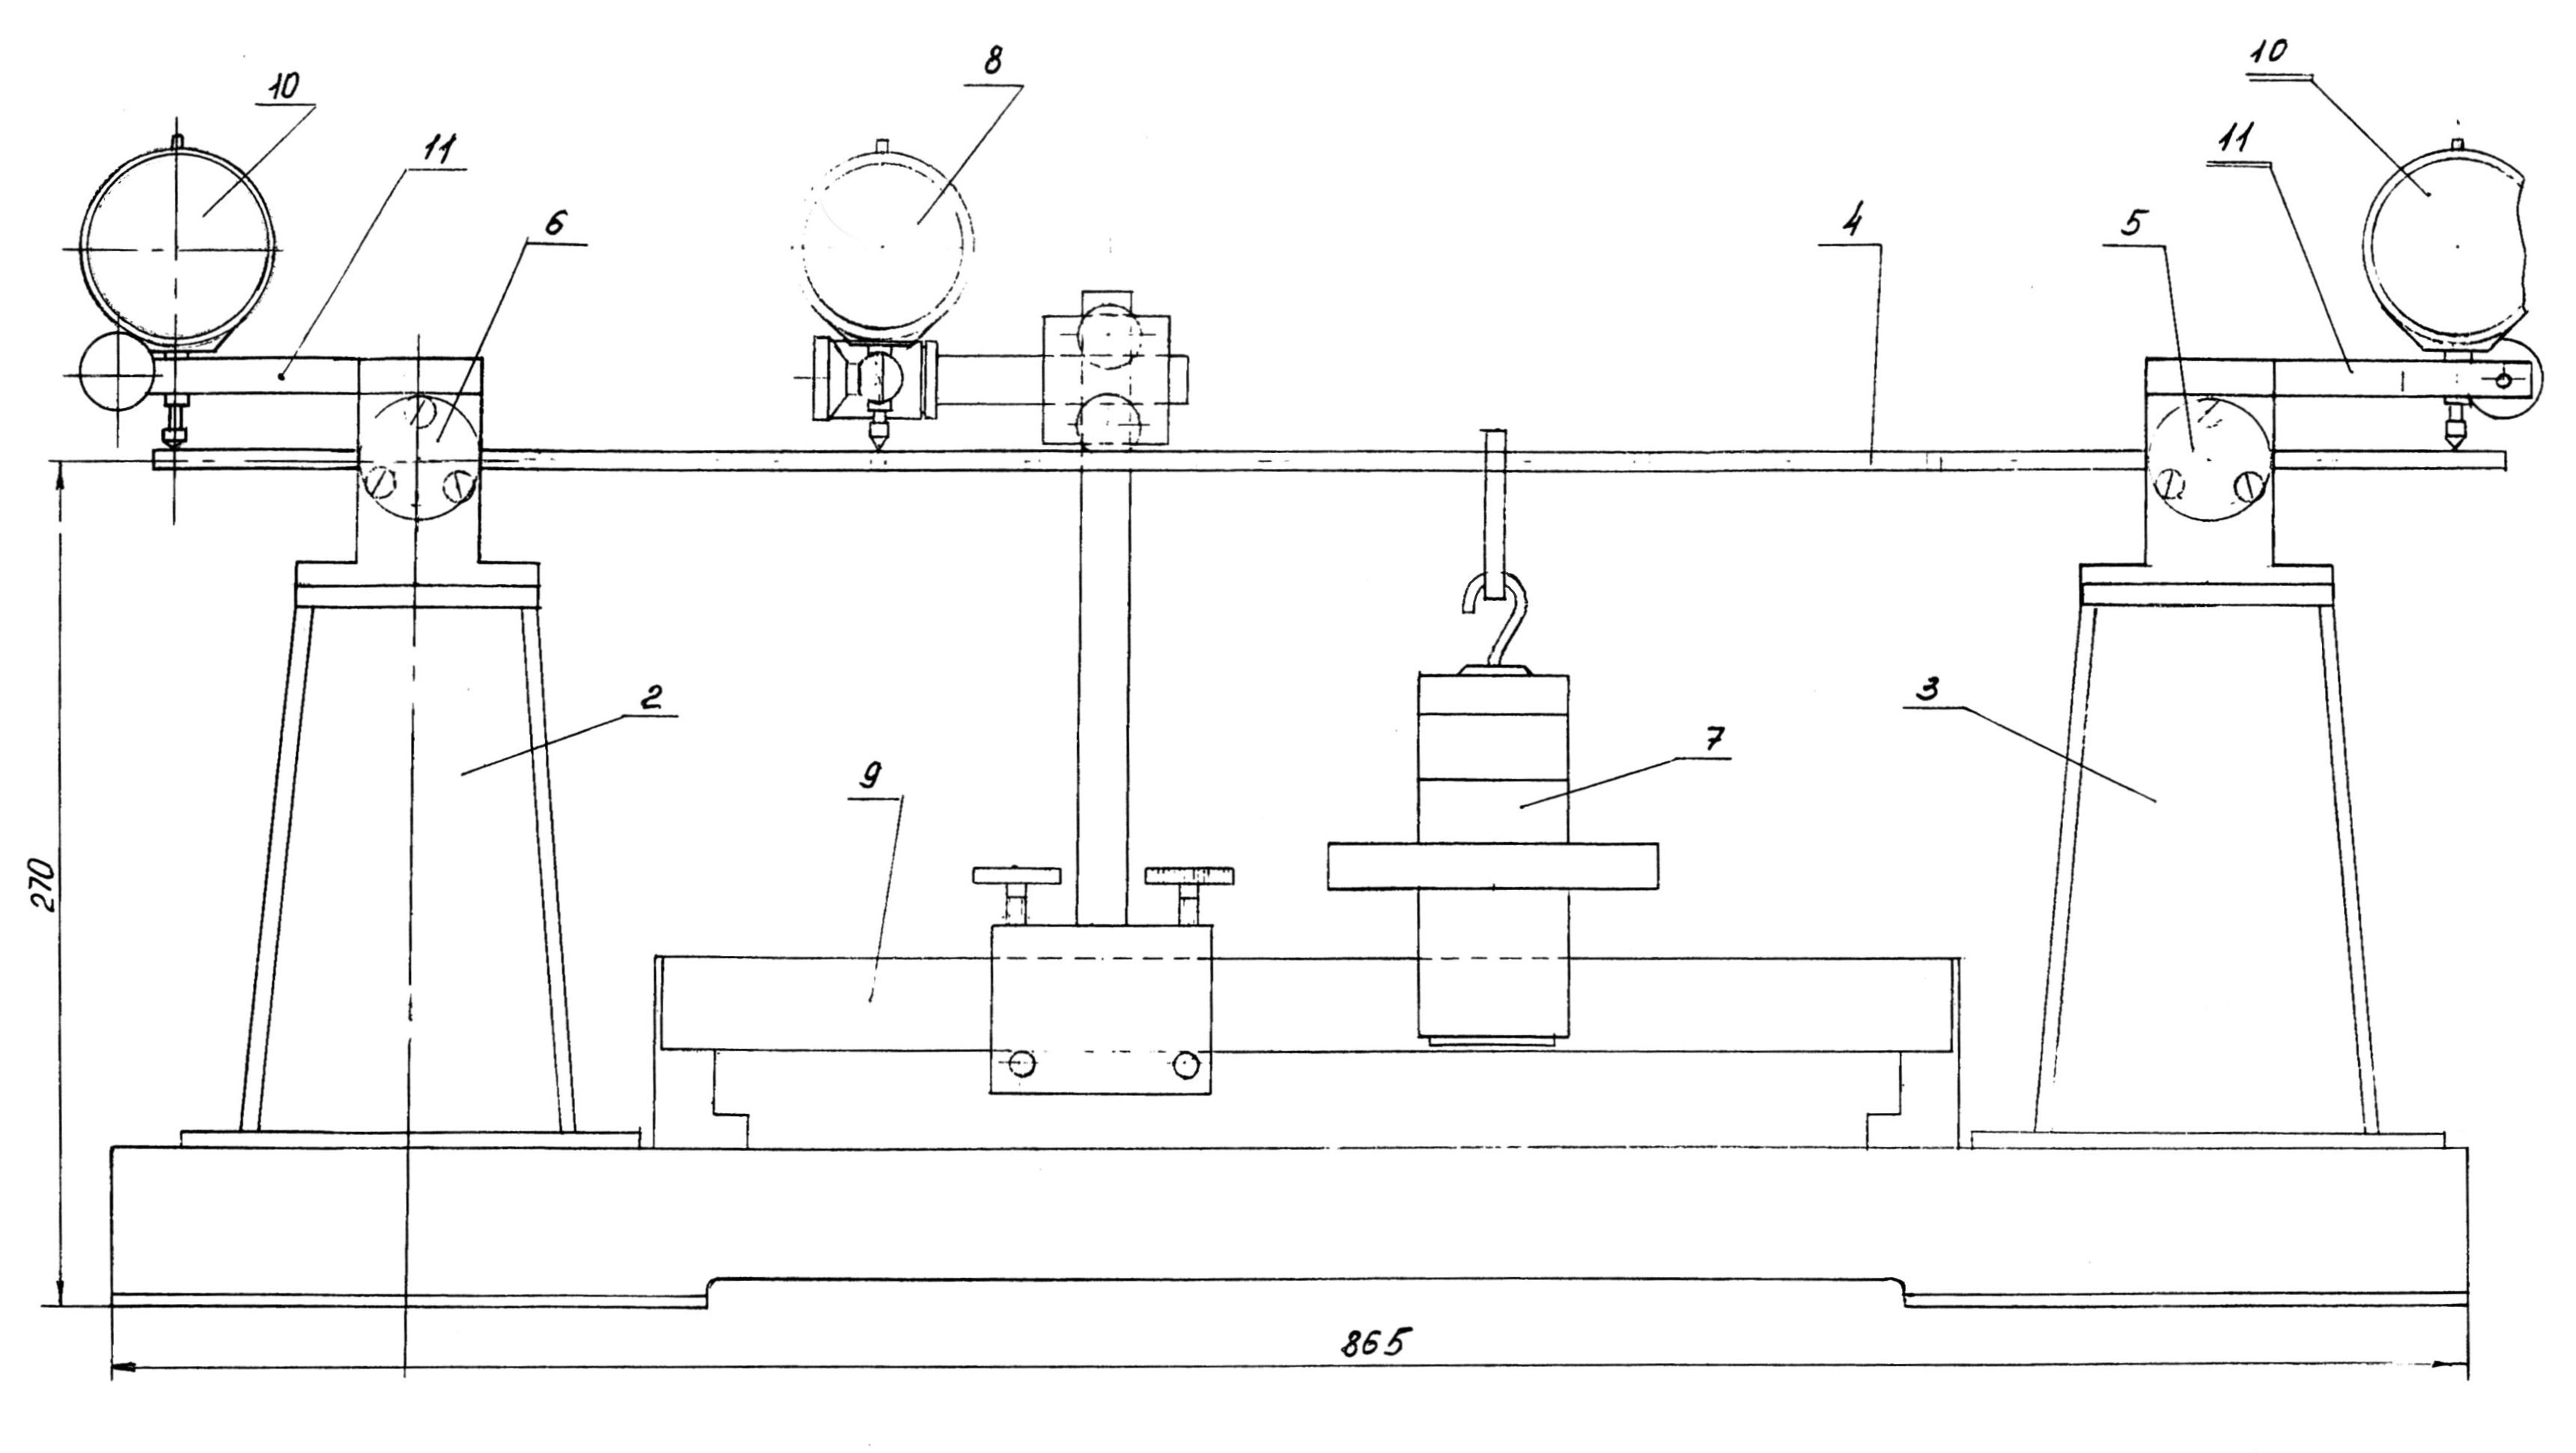
\includegraphics[width = 16cm]{image_1.png}
        \caption{Схема установки.}
        \label{im1}
    \end{figure}
    
    \newpage
    
    \section{Теоретические исследования}
    
    \subsection{Описание изгиба балки}
    
    Под изгибом понимают такой вид деформации, при котором в поперечных сечениях исследуемого образца возникают изгибающие моменты. Стержень, работающий на изгиб, обычно называют балкой. В результате деформации каждое из сечений занимает новое положение: их центры тяжести получают вертикальные $\nu$ и горизонтальные $u$ линейные перемещения, а сами сечения поворачивается на угол $\theta$ вокруг нейтральной оси~--~продольного сечения. в котором отсутствуют растяжение и сжатие (рис.~\ref{im2}).
    
    \begin{figure}[h]
        \centering
        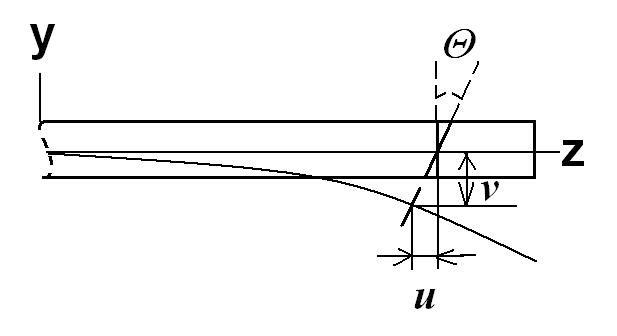
\includegraphics[width = 10cm]{image_2.png}
        \caption{Линейные и угловые перемещения при изгибе.}
        \label{im2}
    \end{figure}
    
    В сопротивлении материалов горизонтальными перемещениями $u$ пренебрегают и изучают прогибы $\nu$ и повороты $\theta$. Дифференциальное уравнение, описывающее изгиб балки известно:
    \begin{equation}
        \nu'' = \frac{d^{2}y}{dz^{2}} = \frac{M(z)}{EI},
        \label{eq1}
    \end{equation}
    где $M(z)$~--~распределение изгибающих моментов по длине образца, $I$~--~момент инерции поперечного сечения балки, $y$~--~координата по высоте сечения. Для балки прямоугольного поперечного сечения момент инерции равен (рис.~\ref{im3}):
    \begin{equation}
        I = \int_{F} y^{2} dF = \frac{bh^{3}}{12}.
        \label{eq2}
    \end{equation}
    
    Интегрируя выражение (\ref{eq1}), получим зависимость от координаты $z$ угла поворота $\theta$, а интегрируя второй раз~--~прогиба $\nu$. Константы интегрирования можно определить из условий отсутствия прогиба на шарнирных опорах.
    
    Изгибающий момент $M$ в сечении $z$ численно равен сумме моментов всех внешних сил (включая силы реакции в опорах), действующих по одну сторону от рассматриваемого сечения. При этом изгибающий момент считается положительным, если элемент изгибается выпуклостью вниз. Распределение какой-либо величины по длине балки в сопротивлении материалов называется эпюрой.
    
    \newpage
    
    \begin{figure}[h]
        \centering
        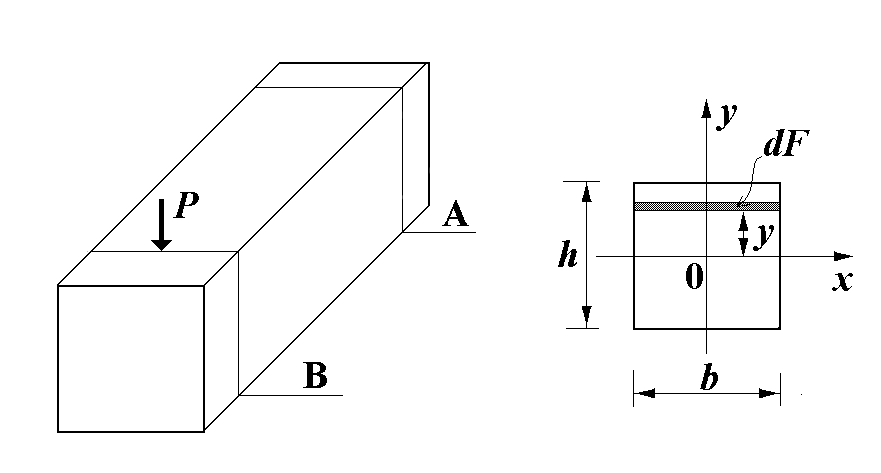
\includegraphics[width = 12cm]{image_3.png}
        \caption{К определению момента инерции сечения.}
        \label{im3}
    \end{figure}
    
    \subsection{Расчет изгиба балки}
    
    Мы предполагаем, что нам известны все геометрические размеры балки и установки, материал балки, величина прикладываемого усилия. В нашей задаче (рис.~\ref{im4}) будем считать известными расстояния $a_{1}$, $a_{2}$, $a_{3}$, нагрузку $P$, момент инерции $I$ поперечного сечения балки и модуль Юнга $E$ материала балки. Предполагаем, что координаты $a_{1}$ и $a_{3}$ соответствуют местам крепления балки, а $a_{2}$ соответствует точке приложения силы.
    
    Наш стержень имеет несколько участков нагружения (рис.~\ref{im4}), поэтому определение произвольных постоянных приводит к решению системы уравнений с большим числом неизвестных, что связано с громоздкими вычислениями. Мы применим <<метод Бубнова>> интегрирования дифференциального уравнения упругой линии, что сведет задачу к определению лишь двух постоянных интегрирования.
    
    \begin{figure}[h]
        \centering
        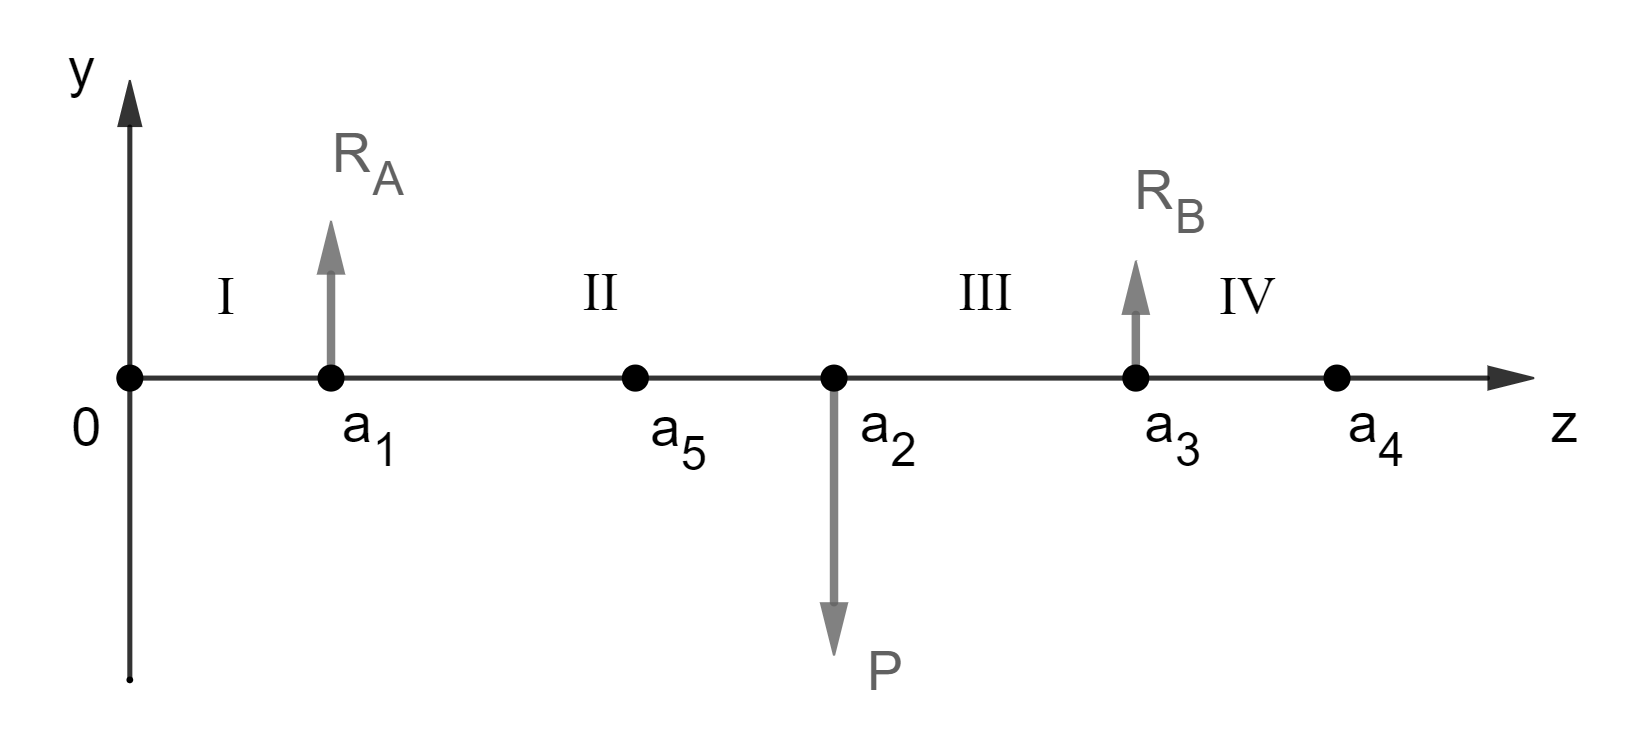
\includegraphics[width = 14cm]{image_4.png}
        \caption{Схема нагружения балки.}
        \label{im4}
    \end{figure}
    
    Для решения задачи проинтегрируем уравнение (\ref{eq1}) один и два раза соответственно, используя метод Бубнова, получим уравнения для изгиба и для отклонения в четырех областях с двумя постоянными интегрирования, которые соответствуют начальному смещению $y_{0}$ и начальному углу отклонения $\theta_{0}$ балки:
    \begin{equation}
        \begin{aligned}
            (I) \quad &\Rightarrow \quad 
            \begin{cases}
                \displaystyle \theta(z) = \theta_{0} \\
                \displaystyle y(z) = y_{0} + \theta_{0}z \\
            \end{cases}, \\
            (II) \quad &\Rightarrow \quad 
            \begin{cases}
                \displaystyle \theta(z) = \frac{1}{EI} \bigg( R_{A} \frac{(z - a_{1})^{2}}{2} \bigg) + \theta_{0} \vspace{0.2cm} \\
                \displaystyle y(z) = \frac{1}{EI} \bigg( R_{A} \frac{(z - a_{1})^{3}}{6} \bigg) + y_{0} + \theta_{0}z \\
            \end{cases}, \\
            (III) \quad &\Rightarrow \quad
            \begin{cases}
                \displaystyle \theta(z) = \frac{1}{EI} \bigg( R_{A} \frac{(z - a_{1})^{2}}{2} - P \frac{(z - a_{2})^{2}}{2} \bigg) + \theta_{0} \vspace{0.2cm} \\
                \displaystyle y(z) = \frac{1}{EI} \bigg( R_{A} \frac{(z - a_{1})^{3}}{6} - P \frac{(z - a_{2})^{3}}{6} \bigg) + y_{0} + \theta_{0}z \\
            \end{cases}, \\
            (IV) \quad &\Rightarrow \quad 
            \begin{cases}
                \displaystyle \theta(z) = \frac{1}{EI} \bigg( R_{A} \frac{(z - a_{1})^{2}}{2} - P \frac{(z - a_{2})^{2}}{2} + R_{B} \frac{(z - a_{3})^{2}}{2} \bigg) + \theta_{0} \vspace{0.2cm} \\
                \displaystyle y(z) = \frac{1}{EI} \bigg( R_{A} \frac{(z - a_{1})^{3}}{6} - P \frac{(z - a_{2})^{3}}{6} + R_{B} \frac{(z - a_{3})^{3}}{6} \bigg) + y_{0} + \theta_{0}z \\
            \end{cases}. \\
        \end{aligned}
        \label{eq3}
    \end{equation}
    В данном случае нам требуется найти значения реакций $R_{A}$ и $R_{B}$ опор. Для этого воспользуемся уравнениями статики для сил и моментов:
    \begin{equation}
        \begin{cases}
            R_{A} + R_{B} - P = 0 \\
            a_{1} R_{A} - a_{2} P + a_{3} R_{B} = 0 \\
        \end{cases},
        \label{eq4}
    \end{equation}
    теперь нужно найти значения постоянных $y_{0}$ и $\theta_{0}$, для этого воспользуемся граничными условиями (на опорах значение отклонения балки равно нулю):
    \begin{equation}
        \begin{cases}
            y(a_{1}) = 0 \\
            y(a_{3}) = 0 \\
        \end{cases}.
        \label{eq5}
    \end{equation}
    
    Найдем выражения для постоянных интегрирования и запишем окончательно уравнения балки с учетом уравнений статики. Сначала выразим реакции опор:
    \begin{equation}
        \begin{cases}
            \displaystyle R_{A} = P \cdot \frac{a_{2} - a_{3}}{a_{1} - a_{3}} \vspace{0.2cm} \\
            \displaystyle R_{B} = P \cdot \frac{a_{1} - a_{2}}{a_{1} - a_{3}} \\
        \end{cases}.
        \label{eq6}
    \end{equation}
    Теперь запишем уравнения для поиска постоянных интегрирования:
    \begin{equation}
        \begin{aligned}
        &\begin{cases}
            \displaystyle y_{0} + \theta_{0} a_{1} = 0 \vspace{0.2cm} \\
            \displaystyle y_{0} + \theta_{0} a_{3} = \frac{P}{6EI} \cdot \Big( (a_{2} - a_{3})(a_{3} - a_{1})^{2} + (a_{3} - a_{2})^{3} \Big)\\
        \end{cases} \Rightarrow \\
        \Rightarrow \quad
        &\begin{cases}
            \displaystyle y_{0} = - \frac{P}{6EI} \cdot \frac{a_{1}((a_{2} - a_{3})(a_{3} - a_{1})^{2} + (a_{3} - a_{2})^{3})}{a_{3} - a_{1}} \vspace{0.2cm} \\
            \displaystyle \theta_{0} = \frac{P}{6EI} \cdot \frac{(a_{2} - a_{3})(a_{3} - a_{1})^{2} + (a_{3} - a_{2})^{3}}{a_{3} - a_{1}} \\
        \end{cases}.
        \end{aligned}
        \label{eq7}
    \end{equation}
    В итоге мы нашли все неизвестные величины, теперь достаточно подставить их в уравнения (\ref{eq3}) для угла изгиба $\theta(z)$ и отклонения $y(z)$, чтобы получить окончательное решение задачи об изгибе балки.
    
    \newpage
    
    \section{Эксперимент}
    
    Все расчеты произведены при помощи пакета Matlab, с кодом программы можно ознакомиться отдельно. Эксперимент проводился в два этапа, сначала балка нагружается слева от центрального индикатора, потом справа. На рис.~\ref{im5} изображена схема установки и все ее характерные размеры.
    
    \begin{figure}[h]
    	\centering
    	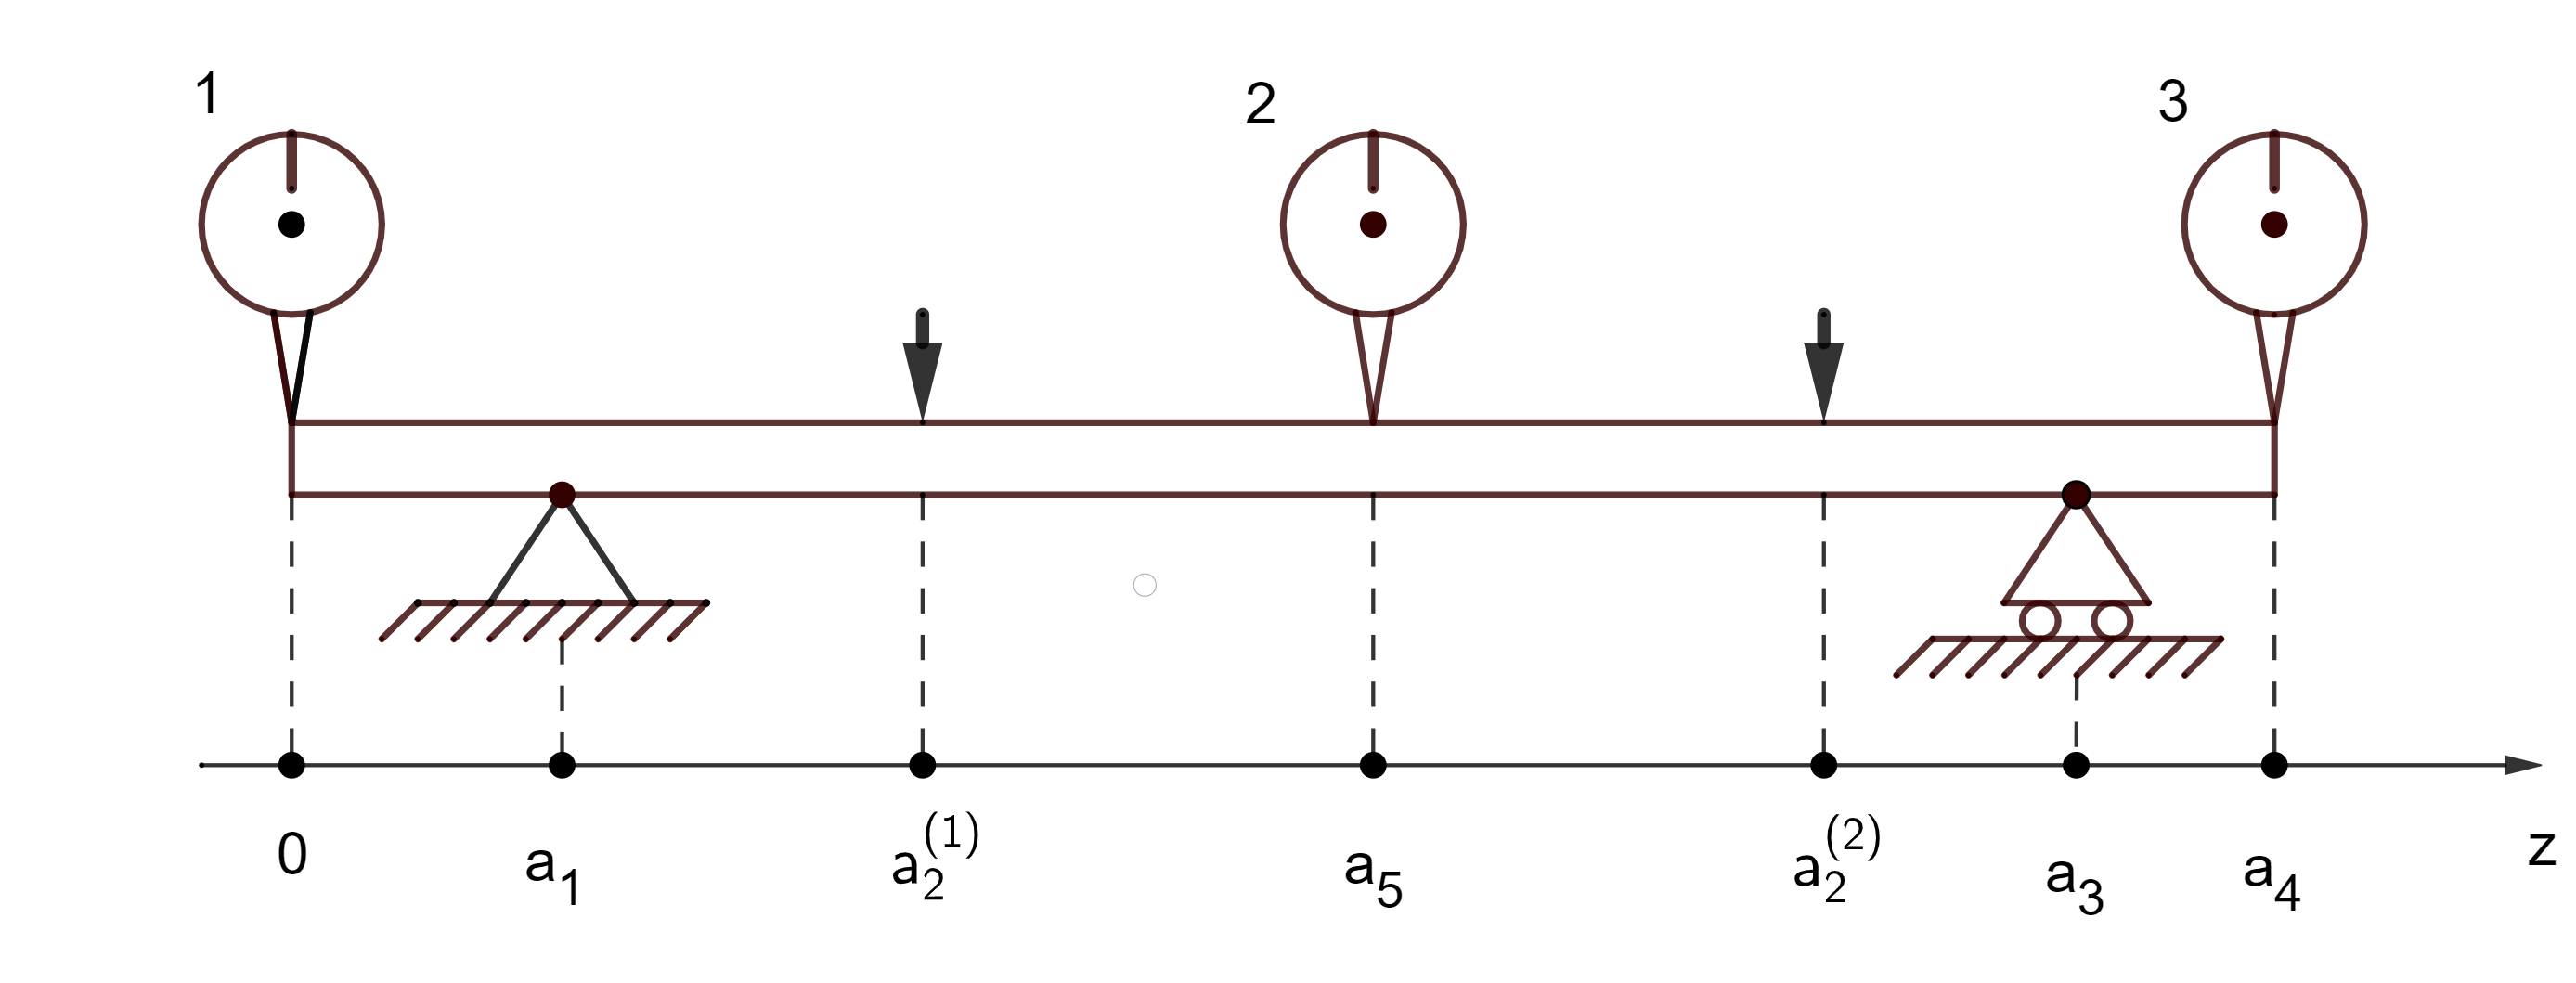
\includegraphics[width = 16cm]{image_5.png}
    	\caption{Измерение длин балки.}
    	\label{im5}
    \end{figure}
    
    Были измерены необходимые расстояния для 2 экспериментов: в 1-ом груз подвешен  в точке $a^{(1)}_{2}$, и во 2-ом груз подвешен в точке $a^{(2)}_{2}$, также произвели замеры высоты $h$ и толщины $b$ балки с оценкой погрешности.
    
    \begin{table}[h]
        \centering
    	\begin{tabular}{|M{2cm}|M{3cm}|M{3cm}|M{3cm}|}
        	\hline
        	Величина & Значение & Погрешность & Размерность \\
        	\hline
        	b & 5.4  & \multirow{2}{*}{$ \pm $0.1} & \multirow{8}{*}{мм} \\
        	h & 36.1 & & \\
        	\cline{1-3}
        	$a_{1}$ & 80  & \multirow{6}{*}{$ \pm $2} & \\
        	$a^{(1)}_{2}$ & 222 & & \\
        	$a^{(2)}_{2}$ & 578 & & \\
        	$a_{3}$ & 779 & & \\
        	$a_{4}$ & 862 & & \\
        	$a_{5}$ & 375  & & \\
            \hline
            $E$ & 200 & -- & ГПа \\
        	\hline
    	\end{tabular}	    
        \label{tb1}
	   \caption{Начальные данные.}    
    \end{table}
    
	Далее провели 2 эксперимента, постепенно нагружая и разгружая балку, снимали показания с индикаторных головок и заносили значения в таблицу, учитывая, что систематическая погрешность измерений для индикатора составляет $\Delta x = 0.5 \cdot 10^{-2}$~мм: 

	\newpage
    
    \begin{table}[h]
        \centering
        \begin{tabular}{|M{1cm}|M{1cm}|M{2cm}|M{2cm}|M{2cm}|M{2cm}|M{2cm}|M{2cm}|}
            \hline
            \multirow{4}{*}{№} & \multirow{3}{*}{P} & \multicolumn{3}{c|}{Опыт №1} & \multicolumn{3}{c|}{Опыт №2} \\
            \cline{3-8}
            & & \multicolumn{3}{c|}{Показания индикаторов} & \multicolumn{3}{c|}{Показания индикаторов} \\
            \cline{3-8}
            & & $y_{1}$ & $y_{2}$ & $y_{3}$ & $y_{1}$ & $y_{2}$ & $y_{3}$ \\
            \cline{2-8}
            & Н &\multicolumn{6}{c|}{$ \cdot 10^{-2} $ мм} \\
        	\hline
        	1 & 1 & 2 & -5 & 1 & 1 & -4 & 1 \\
            2 & 2 & 5 & -10 & 3 & 4 & -12 & 5 \\
       	    3 & 3 & 7 & -15 & 4 & 6 & -19 & 8 \\
        	4 & 5 & 12 & -26 & 7 & 10 & -32 & 14 \\
        	5 & 7 & 17 & -37 & 10 & 15 & -44 & 20 \\
        	6 & 12 & 28 & -63 & 18 & 25 & -76 & 34 \\
        	7 & 7 & 17 & -37 & 11 & 15 & -45 & 21 \\
        	8 & 5 & 12 & -27 & 7 & 11 & -33 & 15 \\
        	9 & 3 & 7 & -16 & 4 & 7 & -20 & 9 \\
            10 & 2 & 5 & -11 & 3 & 4 & -13 & 6 \\
            11 & 1 & 3 & -6 & 1 & 2 & -6 & 3 \\  
            \hline
        \end{tabular}
        \label{tb2}
        \caption{Экспериментальные данные для обоих опытов.}
    \end{table}
    
    Будем опытно искать смещение $y_{0}$ и начальный угол $\theta_{0}$ используя показания индикаторов. Смещение $y_{0}$~--~это есть показание первого индикатора, $\theta_{0}$ найдем по следующей формуле:
    \begin{equation}
        \theta \approx tg\theta = \frac{y_{0}}{a_{1}}.
        \label{eq8}
    \end{equation}
    Теоретический расчет смещений и углов произведем отдельно, а далее сравним значения, которые получились в обоих случаях. Теперь перейдем к анализу первого эксперимента.
    
    \subsection{Опыт №1}
    
    Сначала проведем анализ экспериментальных данных, получим значения смещений и углов. Далее произведем теоретический расчет и сравним его с экспериментальными данными.
    
    \begin{table}[h]
        \centering
        \begin{tabular}{|M{1cm}|M{1cm}|M{1cm}|M{1cm}|M{1cm}|M{1cm}|M{1cm}|M{1cm}|M{1cm}|M{1cm}|M{1cm}|M{1cm}|}
            \hline
            \multirow{2}{*}{№} & $P$ & $y_{1}$ & $\Delta y_{1}$ & $y_{2}$ & $\Delta y_{2}$ & $y_{3}$ & $\Delta y_{3}$ & $\theta_{1}$ & $\Delta \theta_{1}$ & $\theta_{3}$ & $\Delta \theta_{3}$ \\
            \cline{2-12}
            & Н & \multicolumn{6}{c|}{$\cdot 10^{-2} $ мм} & \multicolumn{4}{c|}{$\cdot 10^{-3}$~рад} \\
            \hline
            1 & 1 & 2 & \multirow{6}{*}{0.5} & -5 & \multirow{6}{*}{0.5} & 1 & \multirow{6}{*}{0.5} & -0.25 & 0.06 & 0.12 & 0.06 \\
            2 & 2 & 5 & & -10 & & 3 & & -0.63 & 0.06 & 0.36 & 0.06 \\
            3 & 3 & 7 & & -15 & & 4 & & -0.88 & 0.07 & 0.48 & 0.06 \\
            4 & 5 & 12 & & -26 & & 7 & & -1.50 & 0.07 & 0.84 & 0.06 \\
            5 & 7 & 17 & & -37 & & 10 & & -2.10 & 0.08 & 1.20 & 0.07 \\
            6 & 12 & 28 & & -63 & & 18 & & -3.50 & 0.11 & 2.20 & 0.08 \\ 
            \hline
        \end{tabular}
        \label{tb3}
        \caption{Экспериментальные данные для опыта №1.}
    \end{table}
    
    Теперь мы проведем теоретический расчет, используя результаты, полученные ранее. Будем учитывать погрешность косвенных измерений, но прежде чем перейти к основному расчету, найдем значение момента сечения балки:
    \begin{equation}
        I = 21171 \pm 429~\text{мм}^4.
        \label{eq9}
    \end{equation}
    Теперь составим основную таблицу теоретических результатов:
    
    \begin{table}[h]
        \centering
        \begin{tabular}{|M{0.6cm}|M{0.6cm}|M{1cm}|M{1cm}|M{1.2cm}|M{1cm}|M{1cm}|M{1cm}|M{1.2cm}|M{1cm}|M{1cm}|M{1cm}|}
            \hline
            \multirow{2}{*}{№} & $P$ & $y_{1}$ & $\Delta y_{1}$ & $y_{2}$ & $\Delta y_{2}$ & $y_{3}$ & $\Delta y_{3}$ & $\theta_{1}$ & $\Delta \theta_{1}$ & $\theta_{3}$ & $\Delta \theta_{3}$ \\
            \cline{2-12}
            & Н & \multicolumn{6}{c|}{$\cdot 10^{-2} $ мм} & \multicolumn{4}{c|}{$\cdot 10^{-3}$~рад} \\
            \hline
            1 & 1 & 0.045 & 0.002 & -0.099 & 0.002 & 0.031 & 0.002 & -0.006 & 0.001 & 0.004 & 0.001 \\
            2 & 2 & 0.090 & 0.003 & -0.197 & 0.003 & 0.062 & 0.003 & -0.011 & 0.001 & 0.007 & 0.001 \\
            3 & 3 & 0.134 & 0.005 & -0.296 & 0.005 & 0.093 & 0.005 & -0.017 & 0.001 & 0.011 & 0.001 \\
            4 & 5 & 0.224 & 0.008 & -0.493 & 0.008 & 0.155 & 0.008 & -0.028 & 0.001 & 0.019 & 0.001 \\
            5 & 7 & 0.313 & 0.011 & -0.690 & 0.011 & 0.218 & 0.011 & -0.039 & 0.001 & 0.026 & 0.001 \\
            6 & 12 & 0.537 & 0.019 & -1.183 & 0.019 & 0.373 & 0.019 & -0.067 & 0.002 & 0.045 & 0.002 \\
            \hline
        \end{tabular}
        \label{tb4}
        \caption{Расчетные данные для опыта №1.}
    \end{table}
    
    Далее изобразим графики зависимости отклонения $\nu$ балки в трех точках и изгиба $\theta$ от величины приложенной нагрузки $P$.
    
    \begin{figure}[h!]
        \centering
        \hspace{-2cm}
        \begin{subfigure}{0.4\textwidth}
            \centering
            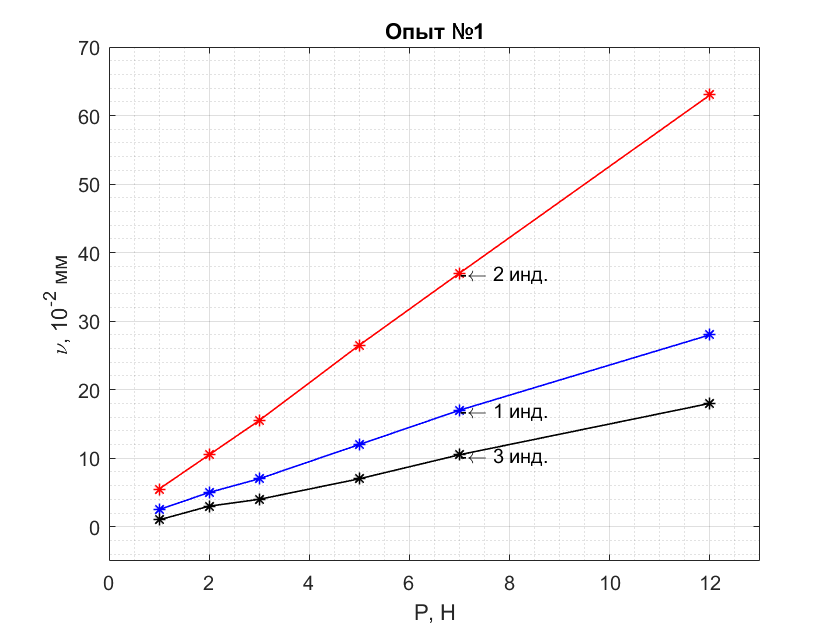
\includegraphics[width = 9cm]{figure_1.png}
        \end{subfigure}
        \hspace{1cm}
        \begin{subfigure}{0.4\textwidth}
            \centering
            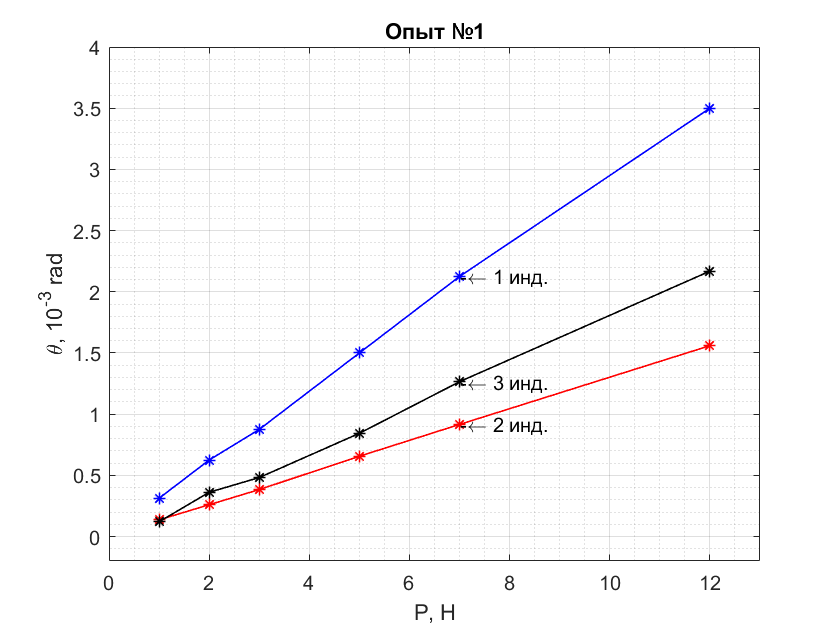
\includegraphics[width = 9cm]{figure_2.png}
        \end{subfigure}
        \caption{\centering Графики зависимости отклонения $\nu$ балки и изгиба $\theta$ от приложенной нагрузки $P$.}
        \label{fig1}
    \end{figure}
    
    Теперь построим эпюры изгибающих моментов и эпюры сил, возникающих в стержне. 
    
    \subsection{Опыт №2}
    
    Теперь рассмотрим ситуацию, когда сила приложена в другом месте балки. Так же как и в первом опыте проведем анализ экспериментальных данных, получим значения смещений и углов. Далее произведем теоретический расчет и сравним его с экспериментальными данными.
    
    \begin{table}[h]
        \centering
        \begin{tabular}{|M{1cm}|M{1cm}|M{1cm}|M{1cm}|M{1cm}|M{1cm}|M{1cm}|M{1cm}|M{1cm}|M{1cm}|M{1cm}|M{1cm}|}
            \hline
            \multirow{2}{*}{№} & $P$ & $y_{1}$ & $\Delta y_{1}$ & $y_{2}$ & $\Delta y_{2}$ & $y_{3}$ & $\Delta y_{3}$ & $\theta_{1}$ & $\Delta \theta_{1}$ & $\theta_{3}$ & $\Delta \theta_{3}$ \\
            \cline{2-12}
            & Н & \multicolumn{6}{c|}{$\cdot 10^{-2} $ мм} & \multicolumn{4}{c|}{$\cdot 10^{-3}$~рад} \\
            \hline
            1 & 1 & 1 & \multirow{6}{*}{0.5} & -4 & \multirow{6}{*}{0.5} & 1 & \multirow{6}{*}{0.5} & -0.13 & 0.06 & 0.12 & 0.06 \\
            2 & 2 & 4 & & -12 & & 5 & & -0.50 & 0.06 & 0.60 & 0.06 \\
            3 & 3 & 6 & & -19 & & 8 & & -0.75 & 0.07 & 0.96 & 0.06 \\
            4 & 5 & 10 & & -32 & & 14 & & -1.30 & 0.07 & 1.70 & 0.07 \\
            5 & 7 & 15 & & -44 & & 20 & & -1.90 & 0.08 & 2.40 & 0.08 \\
            6 & 12 & 25 & & -76 & & 34 & & -3.10 & 0.09 & 4.1 & 0.12 \\ 
            \hline
        \end{tabular}
        \label{tb5}
        \caption{Экспериментальные данные для опыта №2.}
    \end{table}
    
    Далее проведем аналогичный теоретический расчет, но в этот раз учтем, что центральный индикатор находится левее точки приложения нагрузки, то есть мы будем использовать уравнение балки для соответствующего промежутка. Зная это, составим требуемую таблицу.
    
    \begin{table}[h]
        \centering
        \begin{tabular}{|M{0.6cm}|M{0.6cm}|M{1cm}|M{1cm}|M{1.2cm}|M{1cm}|M{1cm}|M{1cm}|M{1.2cm}|M{1cm}|M{1cm}|M{1cm}|}
            \hline
            \multirow{2}{*}{№} & $P$ & $y_{1}$ & $\Delta y_{1}$ & $y_{2}$ & $\Delta y_{2}$ & $y_{3}$ & $\Delta y_{3}$ & $\theta_{1}$ & $\Delta \theta_{1}$ & $\theta_{3}$ & $\Delta \theta_{3}$ \\
            \cline{2-12}
            & Н & \multicolumn{6}{c|}{$\cdot 10^{-2} $ мм} & \multicolumn{4}{c|}{$\cdot 10^{-3}$~рад} \\
            \hline
            1 & 1 & 0.041 & 0.001 & -0.121 & 0.001 & 0.056 & 0.001 & -0.005 & 0.001 & 0.007 & 0.001 \\
            2 & 2 & 0.081 & 0.003 & -0.241 & 0.003 & 0.112 & 0.003 & -0.010 & 0.002 & 0.013 & 0.001 \\
            3 & 3 & 0.122 & 0.004 & -0.362 & 0.004 & 0.168 & 0.004 & -0.015 & 0.002 & 0.020 & 0.001 \\
            4 & 5 & 0.203 & 0.007 & -0.603 & 0.007 & 0.280 & 0.007 & -0.025 & 0.001 & 0.034 & 0.001 \\
            5 & 7 & 0.284 & 0.010 & -0.844 & 0.010 & 0.392 & 0.010 & -0.036 & 0.001 & 0.047 & 0.001 \\
            6 & 12 & 0.487 & 0.017 & -1.447 & 0.017 & 0.672 & 0.017 & -0.061 & 0.002 & 0.081 & 0.002 \\
            \hline
        \end{tabular}
        \label{tb6}
        \caption{Расчетные данные для опыта №2.}
    \end{table}
    
    Далее изобразим графики зависимости отклонения $\nu$ балки в трех точках и изгиба $\theta$ от величины приложенной нагрузки $P$.
    
    \begin{figure}[h!]
        \centering
        \hspace{-2cm}
        \begin{subfigure}{0.4\textwidth}
            \centering
            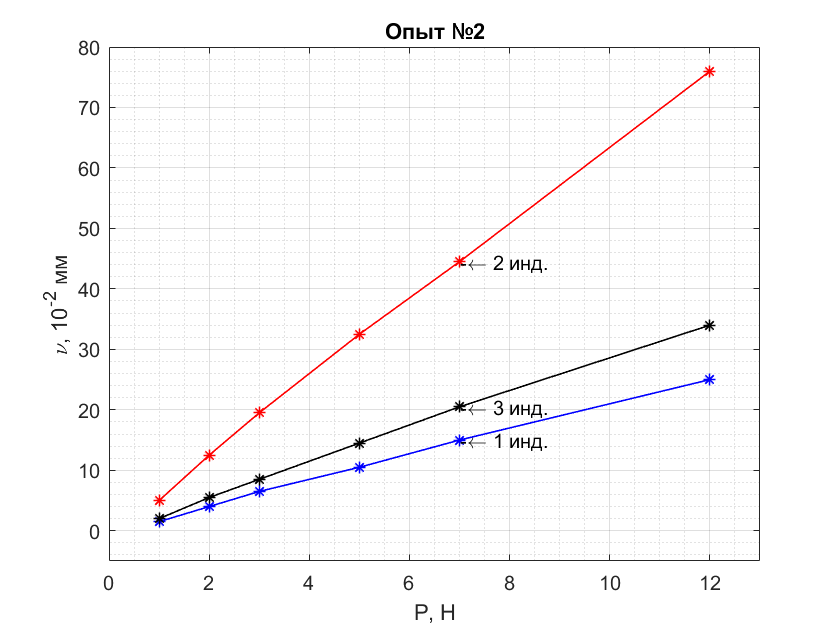
\includegraphics[width = 9cm]{figure_3.png}
        \end{subfigure}
        \hspace{1cm}
        \begin{subfigure}{0.4\textwidth}
            \centering
            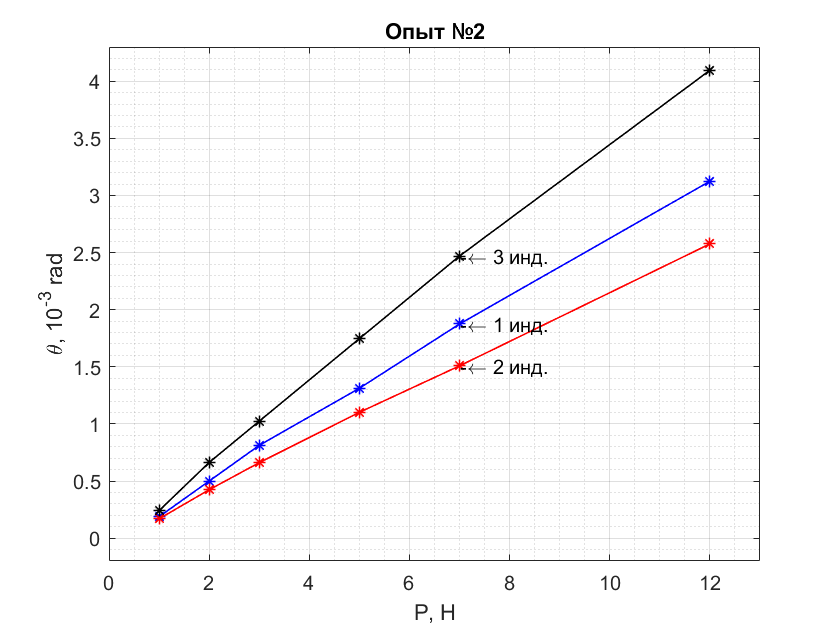
\includegraphics[width = 9cm]{figure_4.png}
        \end{subfigure}
        \caption{\centering Графики зависимости отклонения $\nu$ балки и изгиба $\theta$ от приложенной нагрузки $P$.}
        \label{fig2}
    \end{figure}
    
    Теперь построим эпюры изгибающих моментов и эпюры сил, возникающих в стержне.
    
    \newpage
    
    \section{Выводы}
    
    

\end{document}
